\chapter{Theoretical Framework}
\label{chap:theory}
Some theoretical basics.

\section{The Standard Model of Particle Physics}
\label{sec:SM}

Describe the SM.


\subsection{The WbWb process in the Standard Model}

Representative Feynman diagrams of the two dominant process are depicted in Figure~\ref{fig:wbwb_tt:feynman}.
Contributions from diboson production in association with a $b$ quark are found to be negligible.

\begin{figure}[ht!]
	\centering
	\begin{subfigure}[b]{0.3\linewidth}
		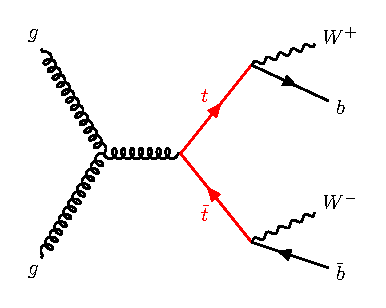
\includegraphics[width=.9\linewidth, page=1]{figures/WbWb/feynman_WbWb.pdf}
		\caption{\ttbar production via gluon-gluon fusion.}
		\label{fig:wbwb:feynman_tt_gg}
	\end{subfigure}\hfill%
	\begin{subfigure}[b]{0.3\linewidth}
		\includegraphics[width=.9\linewidth, page=2]{figures/WbWb/feynman_WbWb.pdf}
		\caption{\ttbar production via quark-antiquark annihilation.}
		\label{fig:wbwb:feynman_tt_qq}
	\end{subfigure}\hfill%
	\begin{subfigure}[b]{0.3\linewidth}
		\includegraphics[width=.7\linewidth, page=3]{figures/WbWb/feynman_WbWb.pdf}
		\caption{\ttbar production in the $t$-channel.}
		\label{fig:wbwb:feynman_tt_tchan}
	\end{subfigure}
	\caption{
    Representative diagrams of \ttbar production modes at the LHC leading to the $WbWb$ final state. \ttbar production at the LHC is predominantly driven by gluon–gluon fusion \subref{fig:wbwb:feynman_tt_gg}, while quark–antiquark annihilation \subref{fig:wbwb:feynman_tt_qq} and the
    $t$-channel process \subref{fig:wbwb:feynman_tt_tchan} occur at significantly lower rates.}
	\label{fig:wbwb_tt:feynman}
\end{figure}


\begin{figure}[ht!]
	\centering
	\begin{subfigure}[b]{0.3\linewidth}
		\includegraphics[width=.9\linewidth, page=5]{figures/WbWb/feynman_WbWb.pdf}
		\caption{$tW$ production via gluon-gluon fusion.}
		\label{fig:wbwb:feynman_tW_gg}
	\end{subfigure}\hfill%
	\begin{subfigure}[b]{0.3\linewidth}
		\includegraphics[width=.9\linewidth, page=6]{figures/WbWb/feynman_WbWb.pdf}
		\caption{$tW$ production via quark-antiquark annihilation.}
		\label{fig:wbwb:feynman_tW_qq}
	\end{subfigure}\hfill%
	\begin{subfigure}[b]{0.3\linewidth}
		\includegraphics[width=.9\linewidth, page=4]{figures/WbWb/feynman_WbWb.pdf}
		\caption{$tW$ production in the $t$-channel.}
		\label{fig:wbwb:feynman_tW_tchan}
	\end{subfigure}
	\caption{
    Representative diagrams with one resonant top quark.
    Possible $tW$ production modes leading to the
    $WbWb$ final state are \subref{fig:wbwb:feynman_tW_gg}~gluon–gluon fusion, \subref{fig:wbwb:feynman_tW_qq} quark–antiquark annihilation or \subref{fig:wbwb:feynman_tW_tchan} the
    $t$-channel process.}
	\label{fig:wbwb_tW:feynman}
\end{figure}



\begin{figure}[ht!]
	\centering
	\begin{subfigure}[t]{0.3\linewidth}
		\includegraphics[width=.9\linewidth, page=7]{figures/WbWb/feynman_WbWb.pdf}
		\caption{$WbWb$ production with an off-shell top quark.}
		\label{fig:wbwb:feynman_nonrestop}
	\end{subfigure}\hfill%
	\begin{subfigure}[t]{0.3\linewidth}
		\includegraphics[width=.9\linewidth, page=8]{figures/WbWb/feynman_WbWb.pdf}
		\caption{$WbWb$ production involving gluon splitting.}
		\label{fig:wbwb:feynman_notop_gg}
	\end{subfigure}\hfill%
	\begin{subfigure}[t]{0.3\linewidth}
		\includegraphics[width=.9\linewidth, page=9]{figures/WbWb/feynman_WbWb.pdf}
		\caption{Quark induced $WbWb$ process without intermediate top quark.}
		\label{fig:wbwb:feynman_notop_qq}
	\end{subfigure}
	\caption{
    Representative diagrams of the $WbWb$ process without resonant top quark, \subref{fig:wbwb:feynman_nonrestop}~with non-resonant (off-shell) top quark or \subref{fig:wbwb:feynman_notop_gg}, \subref{fig:wbwb:feynman_notop_qq} without any top quark involvement.}
	\label{fig:wbwb_nonres:feynman}
\end{figure}


\section{Monte Carlo Event Generators}
\label{sec:MC}

Pythia, Herwig and Sherpa?

